%UNIT 1: QUALITATIVE AND GRAPHICAL APPROACHES
% Is first part of original 01.tex
%%%%%%%%%%%%%%%%%%%%%%%%%%%
%%%% Put the following at the top of each .tex file  %
\pagestyle{fancy}
\renewcommand{\theUnit}{Introduction}
\ifthenelse{\isundefined{\UnitPageNumbers}}{}{\setcounter{page}{1}}
\rhead{Chapter: \theUnit: What Is a Differential Equation?}
\lhead{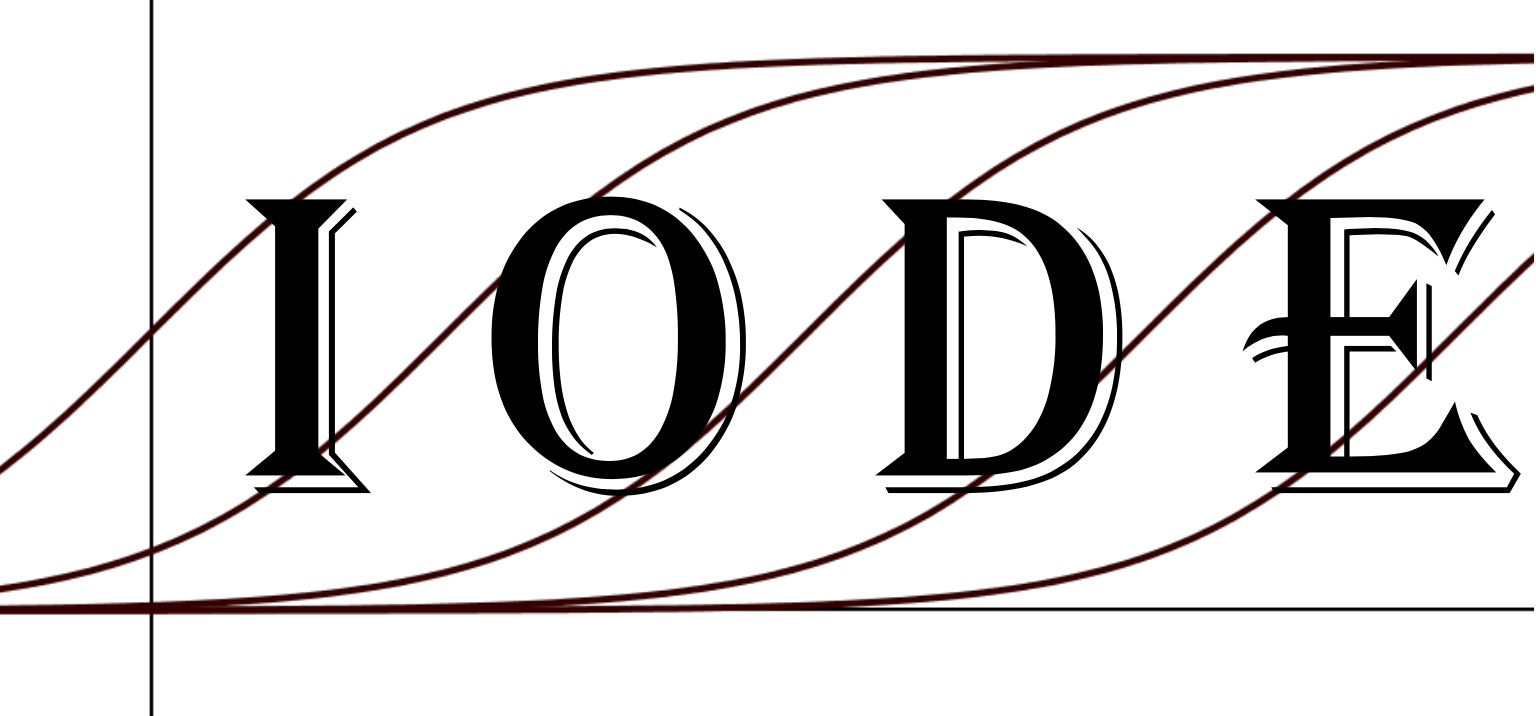
\includegraphics[width=1.25cm]{IODE-logo.png}}
\rfoot{\mypage}
\lfoot{}
\cfoot{}
\fancypagestyle{firstfooter}{\footskip = 50pt}
\renewcommand{\footrulewidth}{.4pt}
%%%%%%%%%%%%%%%%%%%%%%%%%%%
\vspace*{-20pt} \thispagestyle{firstfooter}
\pagebegin{Bees and Flowers}

Often scientists use rate of change equations in their study of population growth for one or more species. In this problem we study systems of rate of change equations designed to inform us about the future populations for two species that are either competitive (that is, both species are \textsl{harmed by} interaction) or cooperative (that is, both species \textsl{benefit from} interaction).
\vs
\begin{enumerate}
\item Which system of rate of change equations below describes a situation where the two species compete and which system describes cooperative species? Explain your reasoning. \label{01problem1}

	\begin{center}
(i)	$  \displaystyle \begin{aligned}[t]
        \frac{dx}{dt} &= -5x +2xy\\
        \frac{dy}{dt} &= -4y +3xy
        \end{aligned}$	\hspace{1.5in}
    (ii) $  \displaystyle \begin{aligned}[t]
        \frac{dx}{dt} &= 4x -2xy\\
        \frac{dy}{dt} &= 2y - xy
        \end{aligned}$
\end{center}
\end{enumerate}

\clearpage
%%%%%%%%%%%%%%%%%
\pagebegin{A Simplified Situation}

The previous problem dealt with a complex situation with two interacting species. To develop the ideas and tools that we will need to further analyze complex situations like these, we will simplify the situation by making the following assumptions:

\begin{itemize}
\item	There is only one species ({\em e.g.}, fish)
\item	The species has been in its habitat ({\em e.g.}, a lake) for some time prior to what we call $t = 0$
\item	The species has access to unlimited resources ({\em e.g.}, food, space, water) 
\item	The species reproduces continuously

\end{itemize}
\begin{enumerate}[resume]
\item	Given these assumptions for a certain lake containing fish, sketch three possible population versus time graphs: one starting at $P = 10$, one starting at $P = 20$, and the third starting at $P = 30$. \label{01problem2}

\begin{center}
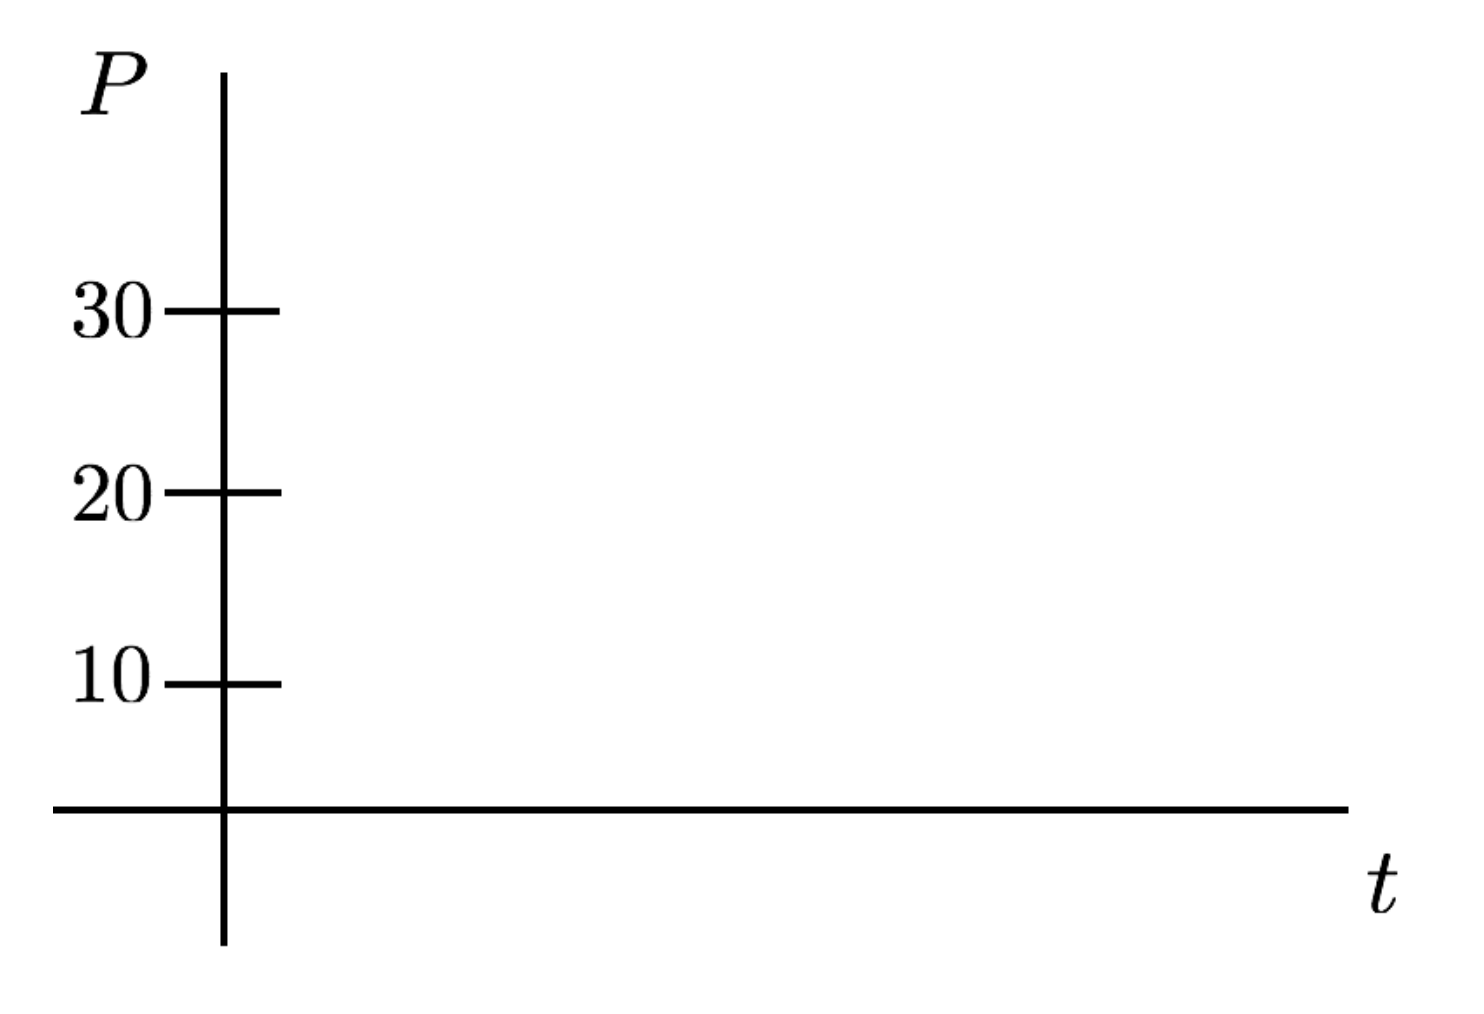
\includegraphics[width=3.5in]{01/01FishGraph.png}
\end{center}
\vspace{-.5in}
\begin{enumerate}
\item	For your graph starting with $P = 10$, how does the slope vary as time increases? Explain. \label{01problem2parta}
\vfill
\item	For a set $P$ value, say $P = 30$, how do the slopes vary across the three graphs you drew? \label{01problem2partb}
\vfill
\end{enumerate}
\item	This situation can also be modeled with a rate of change equation, $\frac{dP}{dt}=something$.  What should the ``something'' be? Should the rate of change be stated in terms of just $P$, just $t$, or both $P$ and $t$? Make a conjecture about the right hand side of the rate of change equation and provide reasons for your conjecture. \label{01problem3}
\end{enumerate}
\vfill

\clearpage
 
%%%%%%%%%%%%%%%%%
\pagebegin{What Exactly is a Differential Equation and What are Solutions?}

A {\bf differential equation} is an equation that relates an unknown function to its derivative(s). Suppose $y = y(t)$ is some unknown function, then a differential equation, would express the rate of change, $\frac{dy}{dt}$, in terms of $y$ and/or $t$. For example, all of the following are \textit{first order} differential equations.  

\[ \frac{dP}{dt}=kP,\qquad \frac{dy}{dt}=y+2t, \qquad \frac{dy}{dt}=t^2+5,\qquad \frac{dy}{dt}=\frac{6y-2}{ty}, \qquad \frac{dy}{dt}=\frac{y^2-1}{t^2+2t}
\]

 Given a differential equation for some unknown function, \textbf{solutions} to this rate of change equation are \textsl{functions} that satisfies the rate change equation. %A constant function that satisfies the differential equation is called an \textbf{equilibrium solution}.
\vs

One way to read the differential equation $\frac{dy}{dt} = y+2t$ aloud you would say, ``dee $y$ dee $t$ equals $y$ plus two times $t$.'' However, this does \textbf{not} relate to the \textsl{meaning} of the solution. 

\begin{enumerate}[resume]
\item \begin{enumerate}
\item Is the function $y=1+t$  a solution to the differential equation $\displaystyle\frac{dy}{dt}=\frac{y^2-1}{t^2+2t}$? How about the function $y=1+2t$?  How about $y = 1$?  Explain your reasoning. \label{01problem4parta} \vfill 

\item	Is the function $y=t^3+2t$    a solution to the differential equation $\displaystyle \frac{dy}{dt}=3y^2+2$?  Why or why not? \label{01problem4partb} \vfill

\end{enumerate}

\item	Figure out all the functions that satisfy the rate of change equation $\displaystyle \frac{dP}{dt}=0.3P$. \vfill

\item	Figure out all of the solutions to the differential equation $\displaystyle\frac{dy}{dt}=t^2+5$. \label{01problem6} \vfill
\end{enumerate}

